\documentclass[12pt]{article}
\usepackage{graphicx} % Required for inserting images
\usepackage[spanish]{babel}
\usepackage{lmodern}
\renewcommand{\familydefault}{\sfdefault}
\usepackage{geometry}
\usepackage{setspace}
\usepackage{float}
\usepackage{xcolor}
\usepackage{amsmath}
\usepackage{tikz}
% Solo una vez se carga hyperref, con tus opciones y el linkcolor
\usepackage[colorlinks=true, urlcolor=blue, linkcolor=black]{hyperref}

\begin{document}
\definecolor{azul}{RGB}{0, 168, 255}
\definecolor{azul2}{RGB}{7, 74, 163}

\begin{titlepage}
    \thispagestyle{empty}
    \newgeometry{left=2cm, right=1cm, top=2cm, bottom=2cm}
    
    % Gráfico de fondo corregido para ser fiable
    \begin{tikzpicture}[overlay, remember picture, fill opacity=0.7]
        \begin{scope}[shift={(current page.center)}]
            \rotatebox{-45}{\fill[azul2] (5, -15) rectangle (12, 15);}
            \rotatebox{-45}{\fill[azul] (3, -15) rectangle (5, 15);}
        \end{scope}
    \end{tikzpicture}
    
    \begin{spacing}{1.5}
        {\Huge \bfseries \noindent PRÁCTICA 4}
        \vspace{10pt}

        {\LARGE RELACIONES CON UNA BASE DE DATOS}
        
        \vspace{1cm}
        
        {\Large Equipo:} \\
        {\Large Beltrán Saucedo Axel Alejandro} \\
        {\Large Cerón Samperio Lizeth Montserrat} \\
        {\Large Higuera Pineda Angel Abraham} \\
        {\Large Lorenzo Silva Abad Rey} \\
        {\Large 4BV1.}
    \end{spacing}
    
    \vspace{1.5cm}

    \begin{minipage}{7.5cm} % Ancho ajustado
        {\Large ESCUELA SUPERIOR DE CÓMPUTO}
    \end{minipage}

    \vfill % Empuja el contenido hacia el final de la página

    \begin{flushleft}
        {\Large \color{black}
        % Comando \textbf corregido con llaves
        \textbf{TECNOLOGÍAS PARA EL DESARROLLO DE APLICACIONES WEB}}
        
        \vspace{0.5cm}
        
        13/10/2025
    \end{flushleft}
    \vspace{1cm}
\end{titlepage}

\newpage
\tableofcontents
\newpage

\section{Introducción}
\subsection*{Planteamiento del problema}
Se busca crear una API web cuyo propósito sea gestionar un inventario y optimizar envíos con ayuda del algoritmo genético simple.
Para la gestión del inventario, se debe garantizar lo siguiente:
\begin{itemize}
    \item Permitir crear, leer, actualizar y borrar items, categorías y envíos en una base de datos.
\end{itemize}

Para la optimización de envíos, se debe garantizar lo siguiente:
\begin{itemize}
    \item Ofrecer un endpoint que utilice el AGS para resolver el problema de la mochila. Que calcule la combinación de items que maximiza la ganancia total de un envío sin exceder una capacidad de peso determinada.
\end{itemize}


\subsection*{Propuesta de solución}
La solución propuesta es el desarrollo de una API con FastAPI para la lógica de negocio y SQLModel para la gestión de la base de datos.
Componentes clave de la solución:
\begin{itemize}
    \item \textbf{SQLModel:} Para definir la estructura de la base de datos estableciendo categoría, item y envío como entidades principales.
    \item \textbf{endpoints (URLs):} Para crear, leer, actualizar y borrar items, categorías y envíos.
    \item \textbf{Algoritmo Génetico:} Realizará el calculo. Simulando un proceso de evolución para encontrar la mejor combinación de items que da la mayor ganancia total sin superar la capacidad.
\end{itemize}

\section{Fundamentos Teóricos}

Para la correcta creacion de nuestra práctica, es importante que entendamos las relaciones entre las tecnologías y los conceptos que ya revisados para la creación de una API, esta vez implementando persistencia de datos.


\subsection*{Entorno de Trabajo y Herramientas Principales}
\begin{itemize}
    \item \textbf{Python:} Es el lenguaje de programación sobre el que se construye toda la lógica de la aplicación. Su sencilla sintaxis y su amplia cantidad de librerías lo hacen ideal para el desarrollo web.\cite{ref2}
    \item \textbf{FastAPI:} Framework web moderno para construir APIs con Python. Sus características más destacadas son la rapidez, la validación de datos automática mediante Pydantic y la generación de documentación interactiva , que fue crucial para probar los endpoints de nuestra API.
    \item \textbf{Uvicorn:} Es un servidor ASGI ultrarrápido, utilizado para ejecutar la aplicación FastAPI. Permite que la API maneje múltiples peticiones de forma asíncrona, mejorando el rendimiento.\cite{ref3}
\end{itemize}

\subsection*{Persistencia de Datos}
La persistencia de datos es la capacidad de un sistema para poder conservar la información posterior de la duración de una sola ejecución. En nuestra practica pasada, los datos eran volátiles, ya que se almacenaban en una lista en memoria. En esta práctica, se implementa la persistencia a través de los siguientes componentes:

\begin{itemize}
    \item \textbf{SQLite:} Es un motor de base de datos relacional, autocontenido y que no requiere un servidor. Almacena toda la base de datos en un único archivo (en nuestro caso, \texttt{database.db}). Es ideal para desarrollo y aplicaciones de pequeña a mediana escala por su simplicidad y portabilidad.
    
    \item \textbf{SQLAlchemy:} Es una librería que funciona como un Mapeador Objeto-Relacional (ORM). Un ORM es una técnica que actúa como un "traductor" entre el código orientado a objetos y las tablas de una base de datos relacional. Permite manipular la base de datos utilizando código Python en lugar de escribir consultas SQL directamente.
    
    \item \textbf{SQLModel:} Es una librería que combina \textbf{SQLAlchemy} y \textbf{Pydantic}, creada por el mismo autor de FastAPI. Permite definir la estructura de los datos, las validaciones y el esquema de la base de datos en una sola clase, reduciendo la duplicación de código y simplificando el desarrollo. En nuestra práctica, las clases como \texttt{Item} son modelos de SQLModel que representan tanto la tabla en la base de datos como los datos que la API recibe y envía.\cite{ref4}
\end{itemize}

\subsection*{Relaciones en Bases de Datos}
\begin{itemize}
    \item \textbf{Relación Unívoca:} Cada valor de clave primaria se relaciona con sólo un registro en la tabla relacionada.
    \item \textbf{Uno a varios:} La tabla de claves primaria sólo contiene un registro que se relaciona con ninguno, uno o varios registros en la tabla relacionada.
    \item \textbf{Varios a varios:} Cada registro en ambas tablas puede estar relacionado con varios registros en la otra tabla. Este tipo de relaciones requieren una tercera tabla, denominada tabla de enlace o asociación, porque los sistemas relacionales no pueden alojar directamente la relación. \cite{ref5}
\end{itemize}

\subsection*{API CRUD}
Una API CRUD es una interfaz de programación que permite Crear, Leer, Actualizar y Borrar datos. \cite{ref6}

\subsubsection*{Algoritmo Genético Simple (AGS)}
Está basado en el proceso genetico de los organismos vivos. 
Los Algoritmos Geneticos usan una analogía directa con el comportamiento natural. 
\begin{itemize}
    \item \textbf{Población:} Trabajan con una poblacion de individuos, cada uno de los cuales representa una solucion factible a un problema dado. A cada individuo se le asigna un valor
 o puntuacion, relacionado con la bondad de dicha solucion. 
    \item \textbf{Fitness:} Cuanto mayor sea la adaptacion de un individuo al problema, mayor
 sera la probabilidad de que el mismo sea seleccionado.
    \item \textbf{Cruzamiento:} Será seleccionado para reproducirse, cruzando su material genetico con otro individuo seleccionado de igual forma. Este cruce producira nuevos individuos descendientes de los anteriores los cuales comparten algunas de las caractersticas de sus padres. Cuanto menor sea la adaptacion de un
 individuo, menor sera la probabilidad de que dicho individuo sea seleccionado para
 la reproduccion, y por tanto de que su material genetico se propague en sucesivas
 generaciones.\cite{ref7}
\end{itemize}
 
 De esta manera se produce una nueva poblacion de posibles soluciones, la cual reemplaza a la anterior y verifica  la interesante propiedad de que contiene una mayor
 proporcion de buenas caractersticas en comparacion con la poblacion anterior. Así a
 lo largo de las generaciones las buenas caractersticas se propagan a travees de la
 poblacion. Favoreciendo el cruce de los individuos mejor adaptados, van siendo explo
radas las areas mas prometedoras del espacio de busqueda. Si el Algoritmo Genetico
 ha sido bien disenado, la poblacion convergera hacia una solucion optima del proble
ma.
\section{Diagrama UML}
\begin{figure}[H]
    \centering
<<<<<<< HEAD
    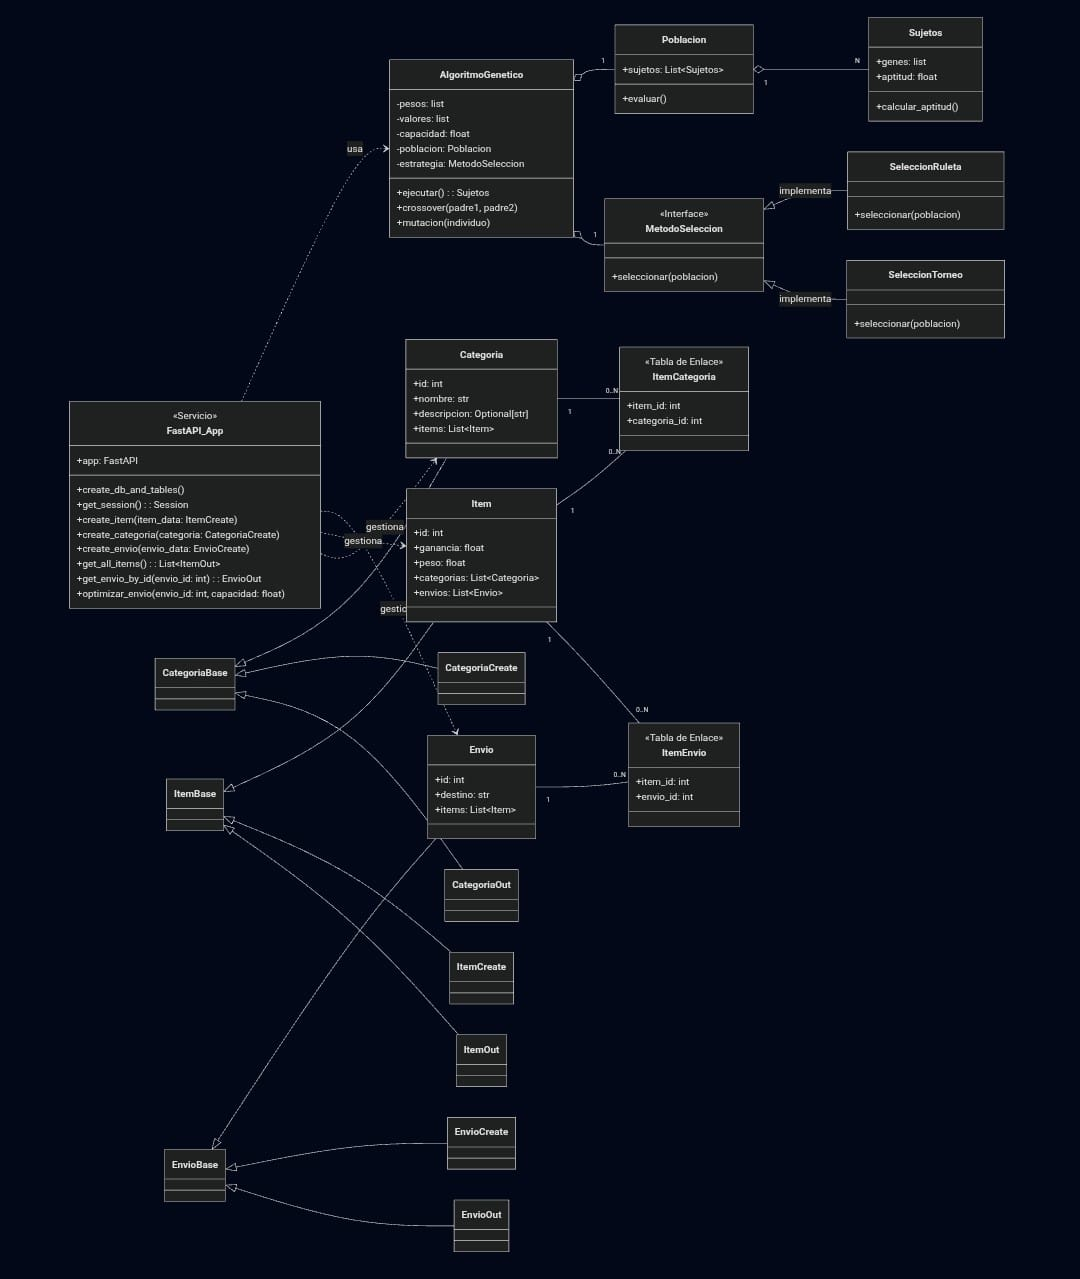
\includegraphics[width=1\textwidth]{Imagenes/diagramauml.jpeg}
=======
    
>>>>>>> 7d864be4b5a5b04fabcc156fd569caccca3a98e0
\end{figure}


\section{Implementación}
\subsection*{Código:}
En esta sección, explicaremos las modificaciones y adiciones clave que transforman la API. El cambio fundamental es la introducción de \textbf{relaciones} en la base de datos, pasando de un solo modelo 'Item' a un sistema de tres modelos interconectados: Item, Categoria, y Envio.

<<<<<<< HEAD
\begin{figure}[H]
    \centering
    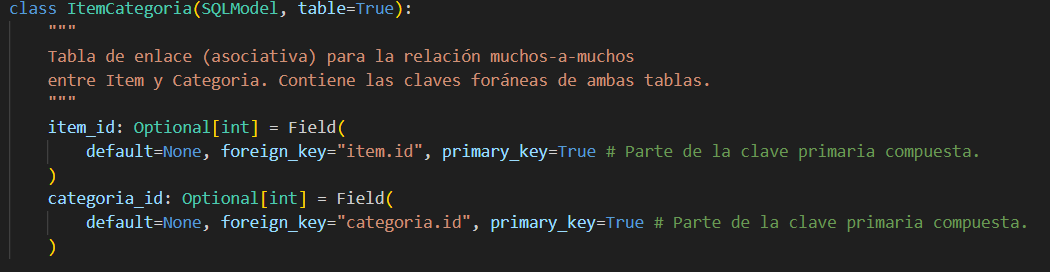
\includegraphics[width=1\textwidth]{Imagenes/Prac4_1.1.png}
    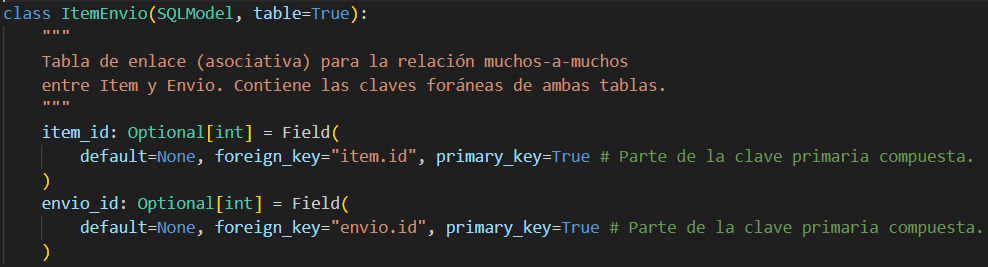
\includegraphics[width=1\textwidth]{Imagenes/Prac4_1.2.png}
    \caption{Definición de las tablas de enlace 'ItemCategoria' y 'ItemEnvio'.}
\end{figure}

La Práctica 4 introduce relaciones de \textbf{muchos a muchos}. Un ítem puede pertenecer a múltiples categorías, y un ítem puede estar en múltiples envíos. Para lograr esto en una base de datos, se requieren "tablas de enlace".
\begin{itemize}
    \item \texttt{ItemCategoria}: Actúa como puente entre 'Item' y 'Categoria'. Contiene 'item\_id' y 'categoria\_id' como claves foráneas y juntas forman la clave primaria.
    \item \texttt{ItemEnvio}: De forma similar, une 'Item' y 'Envio' usando 'item\_id' y 'envio\_id'.
\end{itemize}

\begin{figure}[H]
    \centering
    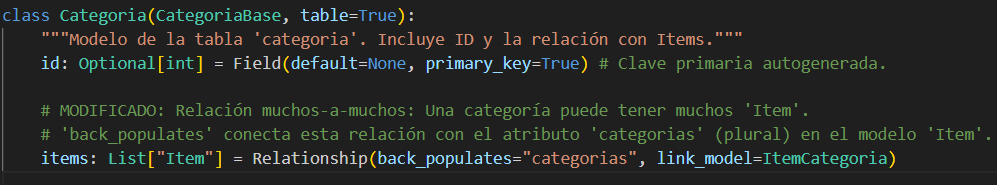
\includegraphics[width=1\textwidth]{Imagenes/Prac4_2.1.png}
    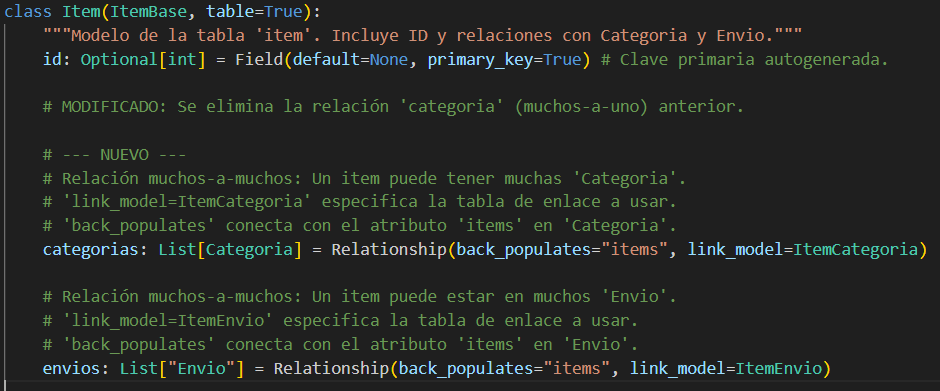
\includegraphics[width=1\textwidth]{Imagenes/Prac4_2.2.png}
    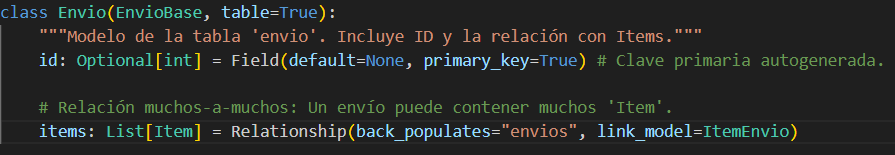
\includegraphics[width=1\textwidth]{Imagenes/Prac4_2.3.png}
    \caption{Modelos de tabla \texttt{Categoria}, \texttt{Item} (modificado) y \texttt{Envio}.}
\end{figure}

Con las tablas de enlace definidas, los modelos principales ahora usan el campo 'Relationship' de SQLModel:
\begin{itemize}
    \item \texttt{Categoria}: Define 'items: List["Item"] = Relationship(...)'.
    \item \texttt{Item}: Es el modelo central en donde se definen dos relaciones: 'categorias: List[Categoria]' y 'envios: List["Envio"]'.
    \item \texttt{Envio}: Define 'items: List[Item] = Relationship(...)'.
\end{itemize}
El parámetro \texttt{link\_model} le dice a SQLModel qué tabla de enlace usar, y \texttt{back\_populates} conecta los dos lados de la relación.

\begin{figure}[H]
    \centering
    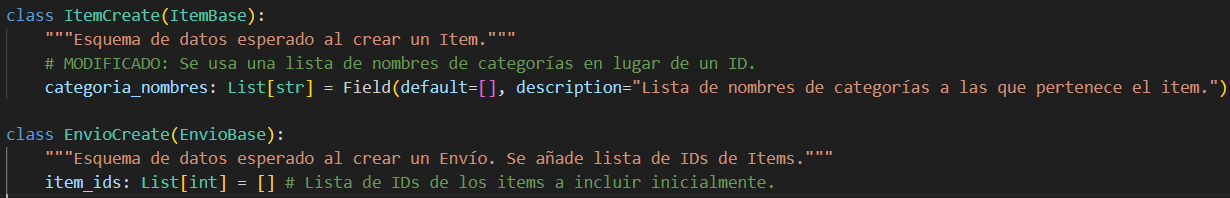
\includegraphics[width=1\textwidth]{Imagenes/Prac4_3.1.png} 
    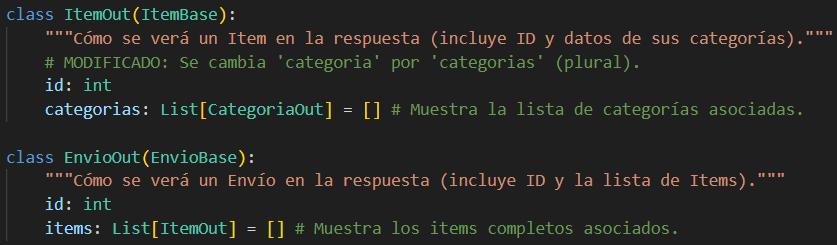
\includegraphics[width=1\textwidth]{Imagenes/Prac4_3.2.png}
    \caption{Modelos de Creación (Input) y Salida (Output).}
\end{figure}

Para manejar estas relaciones en la API, los modelos de "Creación" (Input) y "Salida" (Output) fueron modificados:
\begin{itemize}
    \item \texttt{ItemCreate}: En lugar de pedir un 'categoria\_id', que es lo que se haría en una relación uno-a-muchos, ahora solicita 'categoria\_nombres: List[str]'. Esto resulta mas comodo ya que no se necesitan saber los IDs.
    \item \texttt{EnvioCreate}: Pide una lista de 'item\_ids: List[int]' para asociar items existentes al nuevo envío.
    \item \texttt{ItemOut} y \texttt{EnvioOut}: Se actualizan para mostrar la lista completa de objetos relacionados, dando una respuesta más completa.
\end{itemize}

\begin{figure}[H]
    \centering
    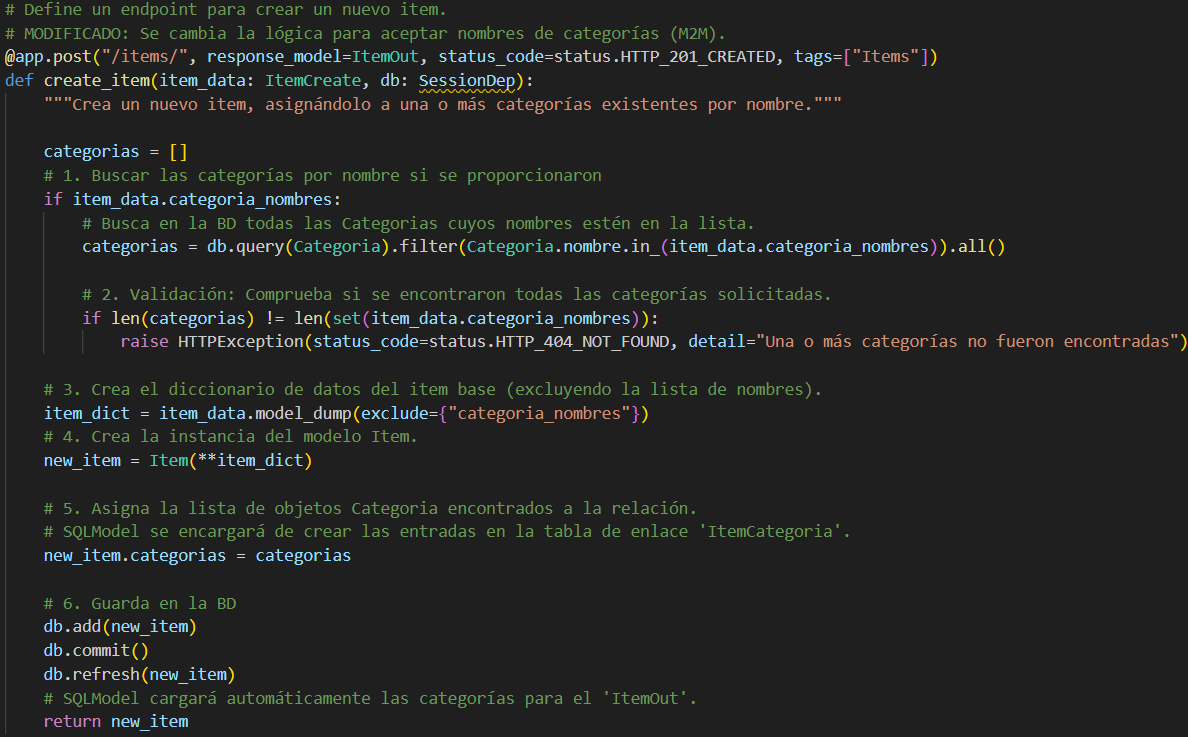
\includegraphics[width=1\textwidth]{Imagenes/Prac4_4.1.png} 
    \caption{Lógica modificada del endpoint POST /items/.}
\end{figure}

La lógica de los endpoints se vuelve un poco mas compleja cuando manejamos las relaciones. Al crear un ítem 'POST \texttt{/items/}', no solo insertamos un registro, sino que ahora debe:
\begin{enumerate}
    \item Recibir la lista de \textbf{nombres} de categorías 'categoria\_nombres'.
    \item Buscar en la base de datos los \textbf{objetos} \texttt{Categoria} que coincidan con esos nombres.
    \item Validar que todas las categorías solicitadas existan.
    \item Crear el nuevo objeto 'Item'.
    \item Asignar la lista de objetos 'Categoria' encontrados al campo 'new\_item.categorias'.
    \item Al hacer 'db.commit()', SQLModel gestiona la tabla de enlace 'ItemCategoria'.
\end{enumerate}
Esta lógica es similar a la aplicada al crear 'Envios' y al actualizar (PATCH) los recursos, donde las listas de relaciones se reemplazan.

\begin{figure}[H]
    \centering
    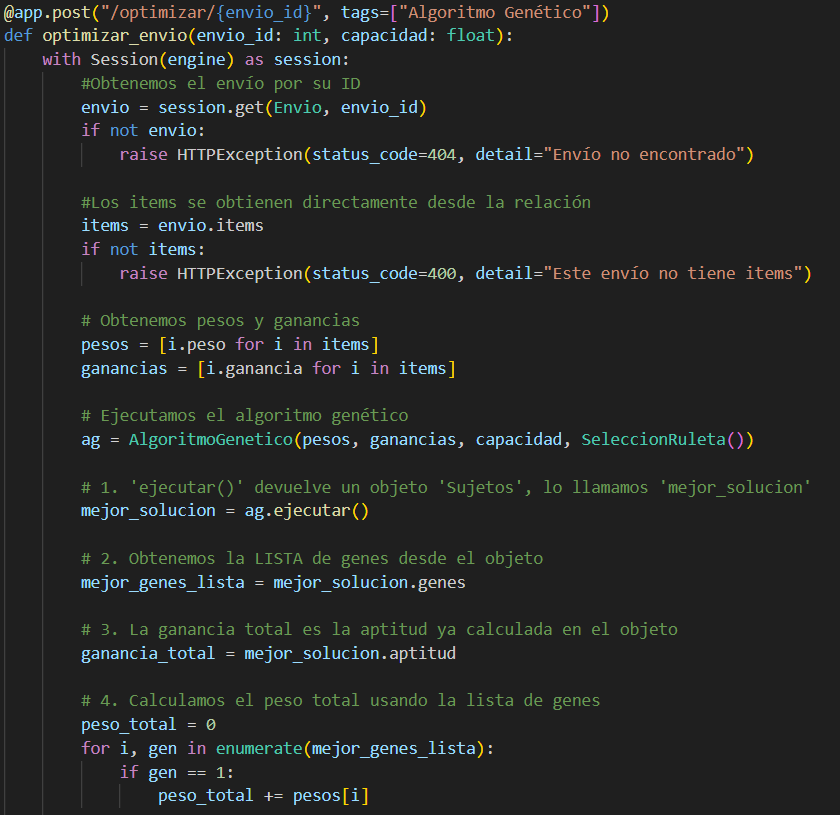
\includegraphics[width=1\textwidth]{Imagenes/Prac4_5.1.png}
    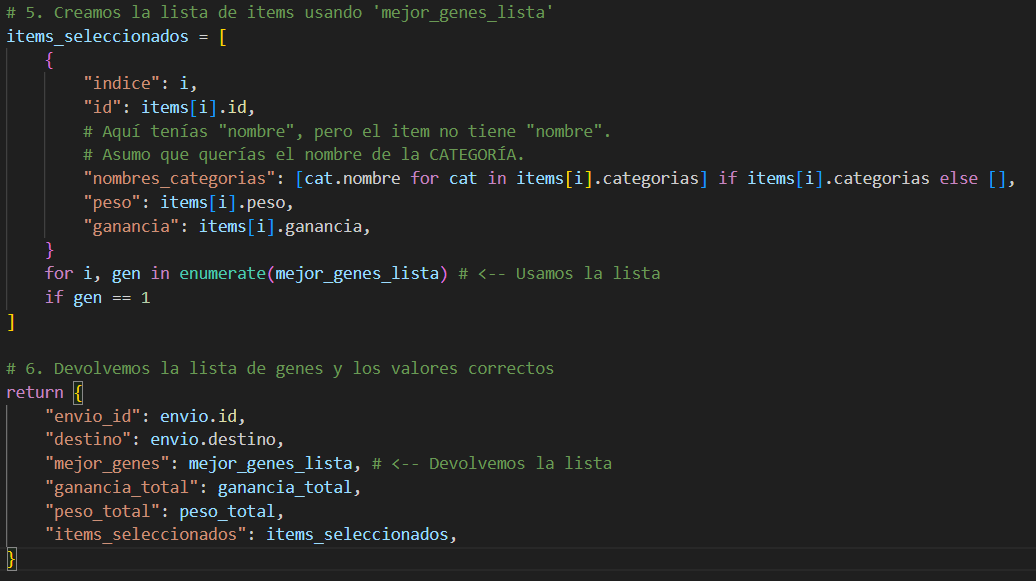
\includegraphics[width=1\textwidth]{Imagenes/Prac4_5.2.png}
    \caption{Nuevo endpoint POST para el Algoritmo Genético.}
\end{figure}

Aqui tenemos la adición más importante, que es el endpoint \texttt{/optimizar/\{envio\_id\}}. Este endpoint integra el algoritmo genético importado desde \texttt{Algoritmo\_genetico.py} con nuestra API de envíos:
\begin{enumerate}
    \item Recibe un 'envio\_id' y una capacidad de peso.
    \item Obtiene el objeto 'Envio' de la base de datos.
    \item Accede a todos los items asociados a ese envío simplemente usando la relación: envio.items.
    \item Extrae los pesos y ganancias de esa lista de items.
    \item Inicializa y ejecuta el 'AlgoritmoGenetico' con esos datos.
    \item La solución se usa para filtrar la lista de items y devolver solo los seleccionados que maximizan la ganancia sin superar la capacidad.
\end{enumerate}
=======

>>>>>>> 7d864be4b5a5b04fabcc156fd569caccca3a98e0

\newpage % Opcional, para que las referencias empiecen en una página nueva

% Añade la línea "Referencias" al índice como si fuera una sección
\addcontentsline{toc}{section}{Referencias}
\begin{thebibliography}{99}

    \bibitem{ref1} IBM. (s.f.). ¿Qué es una API REST? Recuperado el 14 de octubre de 2025, de \url{https://www.ibm.com/mx-es/topics/rest-apis}
    \bibitem{ref2} Python Software Foundation. (s.f.). Acerca de Python™. Resumen Ejecutivo. Recuperado el 14 de octubre de 2025, de \url{https://www.python.org/doc/essays/blurb-es/}
    \bibitem{ref3} Ramírez, S. (s.f.). FastAPI. Recuperado el 14 de octubre de 2025, de \url{https://fastapi.tiangolo.com/es/}
    \bibitem{ref4} Ramírez, S. (s.f.). SQLModel. Recuperado el 14 de octubre de 2025, de \url{https://sqlmodel.tiangolo.com/es/}
    \bibitem{ref5} IBM Control Desk. (s. f.). Relaciones en Bases de Datos. Recuperado el 31 de octubre de 2025, de \url{ https://www.ibm.com/docs/es/control-desk/7.6.1?topic=structure-database-relationships}
    \bibitem{ref6} Jain, A. (2024, 8 septiembre). What is CRUD API? DEV Community. Recuperado el 31 de octubre de 2025, de \url{https://dev.to/ankitjaininfo/what-is-crud-api-502i}
    \bibitem{ref7} Tema 2. Algoritmos genéticos. (s. f.). Departamento de Ciencias de la Computación E Inteligencia Artificial. Recuperado el 31 de octubre de 2025, de \url{http://www.sc.ehu.es/ccwbayes/docencia/mmcc/docs/t2geneticos}

\end{thebibliography}

\end{document}